\section{Metodología}
Para realizar este estudio de revisión sistemática, se estructuró una base de datos analítica y exhaustiva que recopila y documenta de manera detallada las características metodológicas, tecnológicas, de validación y de infraestructura de 213 artículos científicos seleccionados a partir de un proceso riguroso de búsqueda y filtrado. El objetivo de este enfoque es ofrecer una radiografía cuantitativa y cualitativa del estado de la investigación en visión artificial en el transporte.

El proceso de recolección de los artículos científicos siguió las directrices metodológicas de la declaración PRISMA (Preferred Reporting Items for Systematic Reviews and Meta-Analyses). Se realizaron búsquedas estructuradas en las principales bases de datos internacionales de mayor prestigio y relevancia para las ciencias de la computación e ingeniería, específicamente: \textbf{IEEE Xplore}, \textbf{ScienceDirect (Elsevier)}, \textbf{SpringerLink} y \textbf{Scopus}. Las cadenas de búsqueda y las respectivas bases de datos empleadas en el proceso de recolección se resumen en la Tabla~\ref{tab:cadenas_busqueda}.

\begin{table}[htbp]
\centering
\renewcommand{\arraystretch}{1.3}
\caption{Cadenas de Búsqueda y Bases de Datos Utilizadas}
\label{tab:cadenas_busqueda}
\begin{tabular}{@{}l p{6.2cm}@{}}
\toprule
\textbf{Base de Datos} & \textbf{Cadena de Búsqueda (Search Query)} \\
\midrule
IEEE Xplore & \textit{``driver fatigue monitoring''} \textbf{AND} \textit{``computer vision''} \\
ScienceDirect & \textit{``computer vision''} \textbf{AND} \textit{``traffic violation''} \textbf{AND} \textit{``detection''} \\
Scopus & \textit{``YOLO''} \textbf{AND} \textit{``vehicle detection''} \textbf{AND} \textit{``intelligent transportation systems''} \\
SpringerLink & \textit{``driver distraction detection''} \textbf{AND} \textit{``deep learning''} \\
\bottomrule
\end{tabular}
\end{table}

A través de esta estrategia de búsqueda inicial, se identificaron un total de \textbf{456 artículos} en las bases de datos mencionadas. Para depurar este conjunto y asegurar la calidad y alineación del corpus final con el alcance del estudio, se aplicaron criterios de inclusión y aceptación/exclusión secuenciales:
\begin{enumerate}
    \item \textbf{Criterios de Inclusión:} Publicaciones revisadas por pares, escritas en inglés o español, con enfoque directo en aplicaciones de visión artificial o aprendizaje automático para ITS o monitoreo de conductores, y con fecha de publicación comprendida entre 2020 y 2026.
    \item \textbf{Criterios de Aceptación/Exclusión:} Estudios que presentaran resultados experimentales empíricos detallados (con métricas cuantitativas como exactitud, precisión, mAP o FPS) y detalles claros sobre la implementación de hardware y software. Se excluyeron patentes, resúmenes de congresos sin artículo completo, y estudios basados puramente en simulaciones teóricas sin validación empírica con conjuntos de datos reales.
\end{enumerate}

Tras remover duplicados entre las diferentes bases de datos y evaluar la conformidad con los criterios de inclusión y aceptación, se seleccionó un corpus final de \textbf{213 artículos} para el análisis estadístico y cualitativo detallado. El proceso detallado de selección se presenta en la Fig.~\ref{fig:prisma_flow}.

\begin{figure}[htbp]
\centering
\shorthandoff{<}\shorthandoff{>}
\begin{tikzpicture}[node distance=1.2cm, every node/.style={fill=white, font=\scriptsize}, align=center]
  % Estilos de TikZ
  \tikzstyle{box} = [rectangle, draw, fill=blue!5, text width=3.4cm, minimum height=0.8cm, rounded corners=1pt]
  \tikzstyle{sidebox} = [rectangle, draw, fill=red!5, text width=2.8cm, minimum height=0.8cm, rounded corners=1pt]
  \tikzstyle{arrow} = [thick,->,>=stealth]
  % Nodos
  \node (ident) [box] {\textbf{Identificación}\\ Búsqueda inicial en bases de datos ($N = 456$)};
  \node (dup) [sidebox, right=0.3cm of ident] {\textbf{Exclusión Duplicados}\\ Registros eliminados\\ ($N = 104$)};
  \node (screen) [box, below=0.6cm of ident] {\textbf{Cribado (Screening)}\\ Evaluación de título y resumen ($N = 352$)};
  \node (excl_screen) [sidebox, right=0.3cm of screen] {\textbf{Excluidos}\\ Fuera de tema\\ ($N = 89$)};
  \node (elig) [box, below=0.6cm of screen] {\textbf{Elegibilidad}\\ Análisis a texto completo ($N = 263$)};
  \node (excl_elig) [sidebox, right=0.3cm of elig] {\textbf{Excluidos ($N = 50$):}\\ - Sin datos empíricos\\ - Sin hardware/software};
  \node (incl) [box, below=0.6cm of elig] {\textbf{Incluidos}\\ Corpus final de estudios ($N = 213$)};
  % Conexiones
  \draw [arrow] (ident) -- (screen);
  \draw [arrow] (ident) -- (dup);
  \draw [arrow] (screen) -- (elig);
  \draw [arrow] (screen) -- (excl_screen);
  \draw [arrow] (elig) -- (incl);
  \draw [arrow] (elig) -- (excl_elig);
\end{tikzpicture}
\shorthandon{<}\shorthandon{>}
\caption{Diagrama de Flujo del Proceso de Selección de Estudios (Declaración PRISMA).}
\label{fig:prisma_flow}
\end{figure}

La distribución de los 456 registros inicialmente identificados según las bases de datos de procedencia se expone en la Fig.~\ref{fig:db_dist}, evidenciando que ScienceDirect e IEEE Xplore representan los principales repositorios de publicaciones del área.

\begin{figure}[htbp]
\centering
\centerline{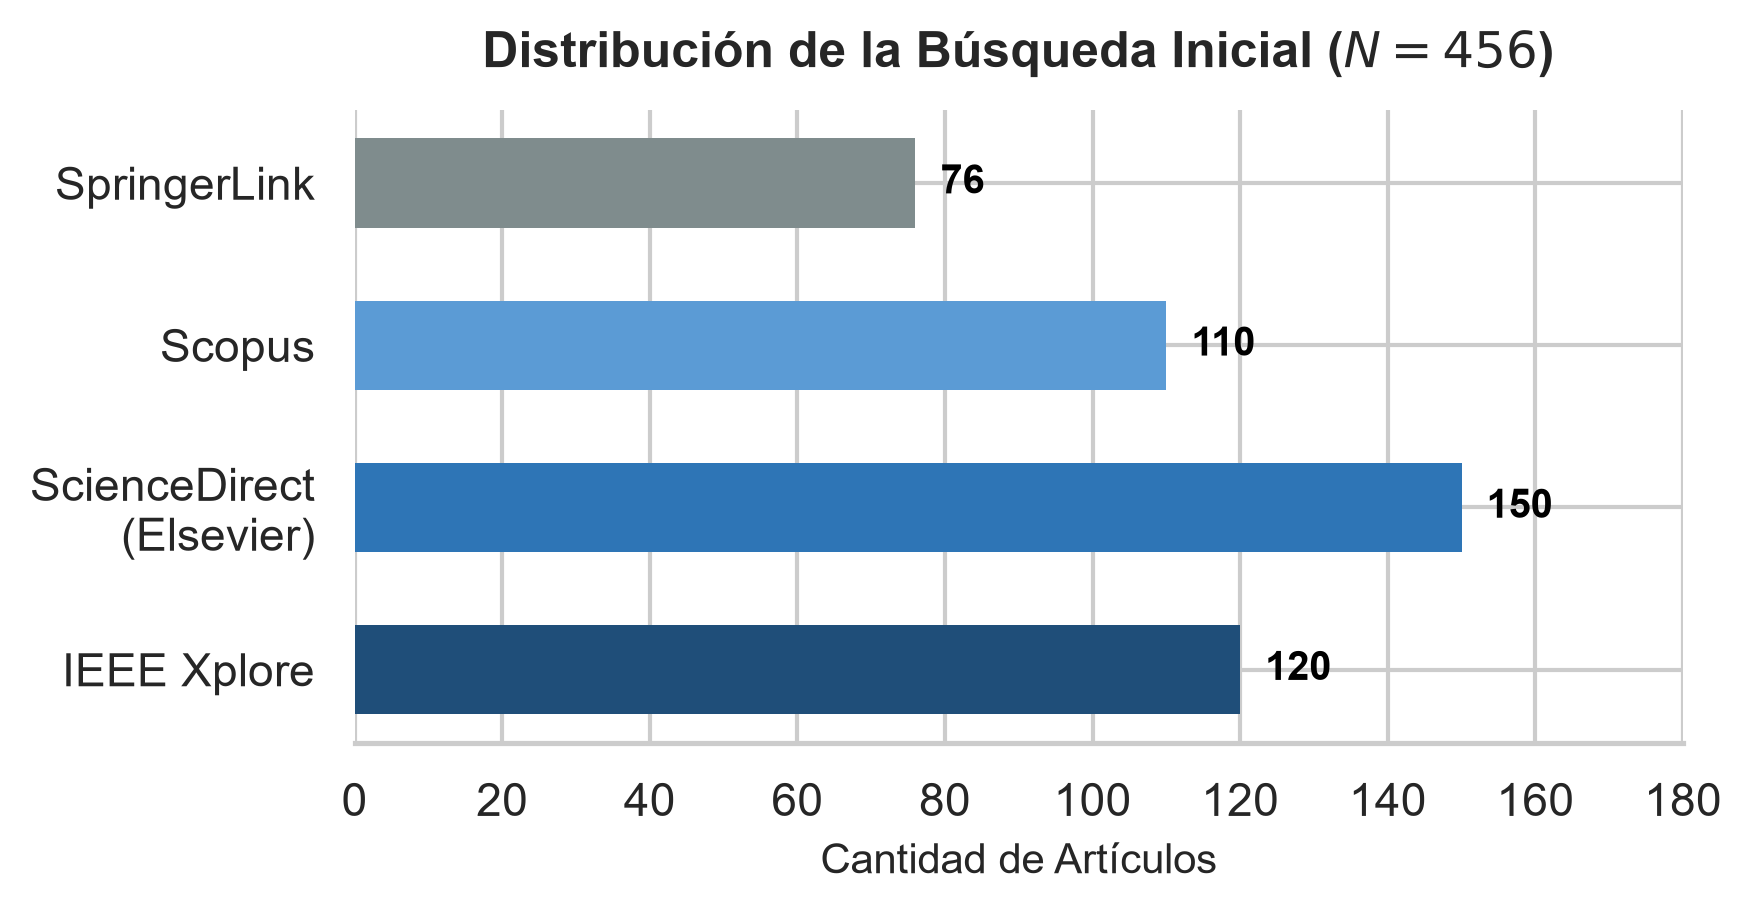
\includegraphics[width=0.48\textwidth]{../graficos/24_prisma_db_dist.png}}
\caption{Distribución de Artículos Encontrados en la Búsqueda Inicial por Base de Datos.}
\label{fig:db_dist}
\end{figure}

\subsection{Preguntas de Investigación y Enfoque PICO}
Para estructurar formalmente el alcance de la revisión sistemática, se formularon los objetivos bajo el marco conceptual PICO (Población, Intervención, Comparación y Resultado/Outcome), el cual se resume en la Tabla~\ref{tab:pico}.

\begin{table}[htbp]
\centering
\renewcommand{\arraystretch}{1.3}
\caption{Estructura del Enfoque PICO de la Revisión}
\label{tab:pico}
\begin{tabular}{@{}p{2.2cm}p{6.2cm}@{}}
\toprule
\textbf{Componente PICO} & \textbf{Descripción} \\
\midrule
\textbf{P}oblación / Contexto & Conductores viales y flujos de tráfico en entornos urbanos y autopistas. \\
\textbf{I}ntervención / Tecnología & Algoritmos de IA y Visión Computacional (Deep Learning, YOLO, CNNs, etc.). \\
\textbf{C}omparación & Enfoques metodológicos (DL, ML, Híbrido, OpenCV) y entornos (CCTV, UAV, Simulador, Vía Real). \\
\textbf{O}utcome (Resultado) & Métricas de desempeño (Accuracy, mAP), latencia (FPS) y viabilidad de despliegue (Edge Computing). \\
\bottomrule
\end{tabular}
\end{table}

Para guiar la recopilación y el análisis cuantitativo de la literatura, se plantearon tres preguntas de investigación fundamentales:
\begin{itemize}
    \item \textbf{PI1:} ¿Cuáles son las principales arquitecturas y enfoques metodológicos de Inteligencia Artificial y Visión por Computadora utilizados para el Monitoreo del Comportamiento de Conductores y los Sistemas de Transporte Inteligentes (ITS) en la literatura científica reciente (2020--2026)?
    \item \textbf{PI2:} ¿Qué entornos experimentales de prueba, plataformas de hardware de despliegue y herramientas de software de implementación predominan en la validación de estas tecnologías viales?
    \item \textbf{PI3:} ¿Cuáles son las limitaciones operativas, sesgos de datos y desafíos técnicos más críticos reportados por los investigadores, y qué direcciones de trabajo futuro se proponen para superarlos?
\end{itemize}

\subsection{Distribución Temporal de las Publicaciones}
El interés investigativo en la convergencia de la inteligencia artificial y el transporte inteligente ha mostrado una trayectoria de crecimiento significativo durante el periodo evaluado (2020--2026). Como se detalla en la Tabla~\ref{tab:dist_anos}, la cantidad de publicaciones anuales experimentó un incremento sostenido, alcanzando su pico de producción científica en el periodo 2024--2025 con un total de 97 trabajos. Este dinamismo refleja la rápida adopción de nuevas arquitecturas de aprendizaje profundo y la disponibilidad de hardware de bajo costo. La Fig.~\ref{fig:linea_publicaciones} ilustra visualmente esta tendencia de crecimiento en el volumen de publicaciones.

\begin{figure}[htbp]
\centerline{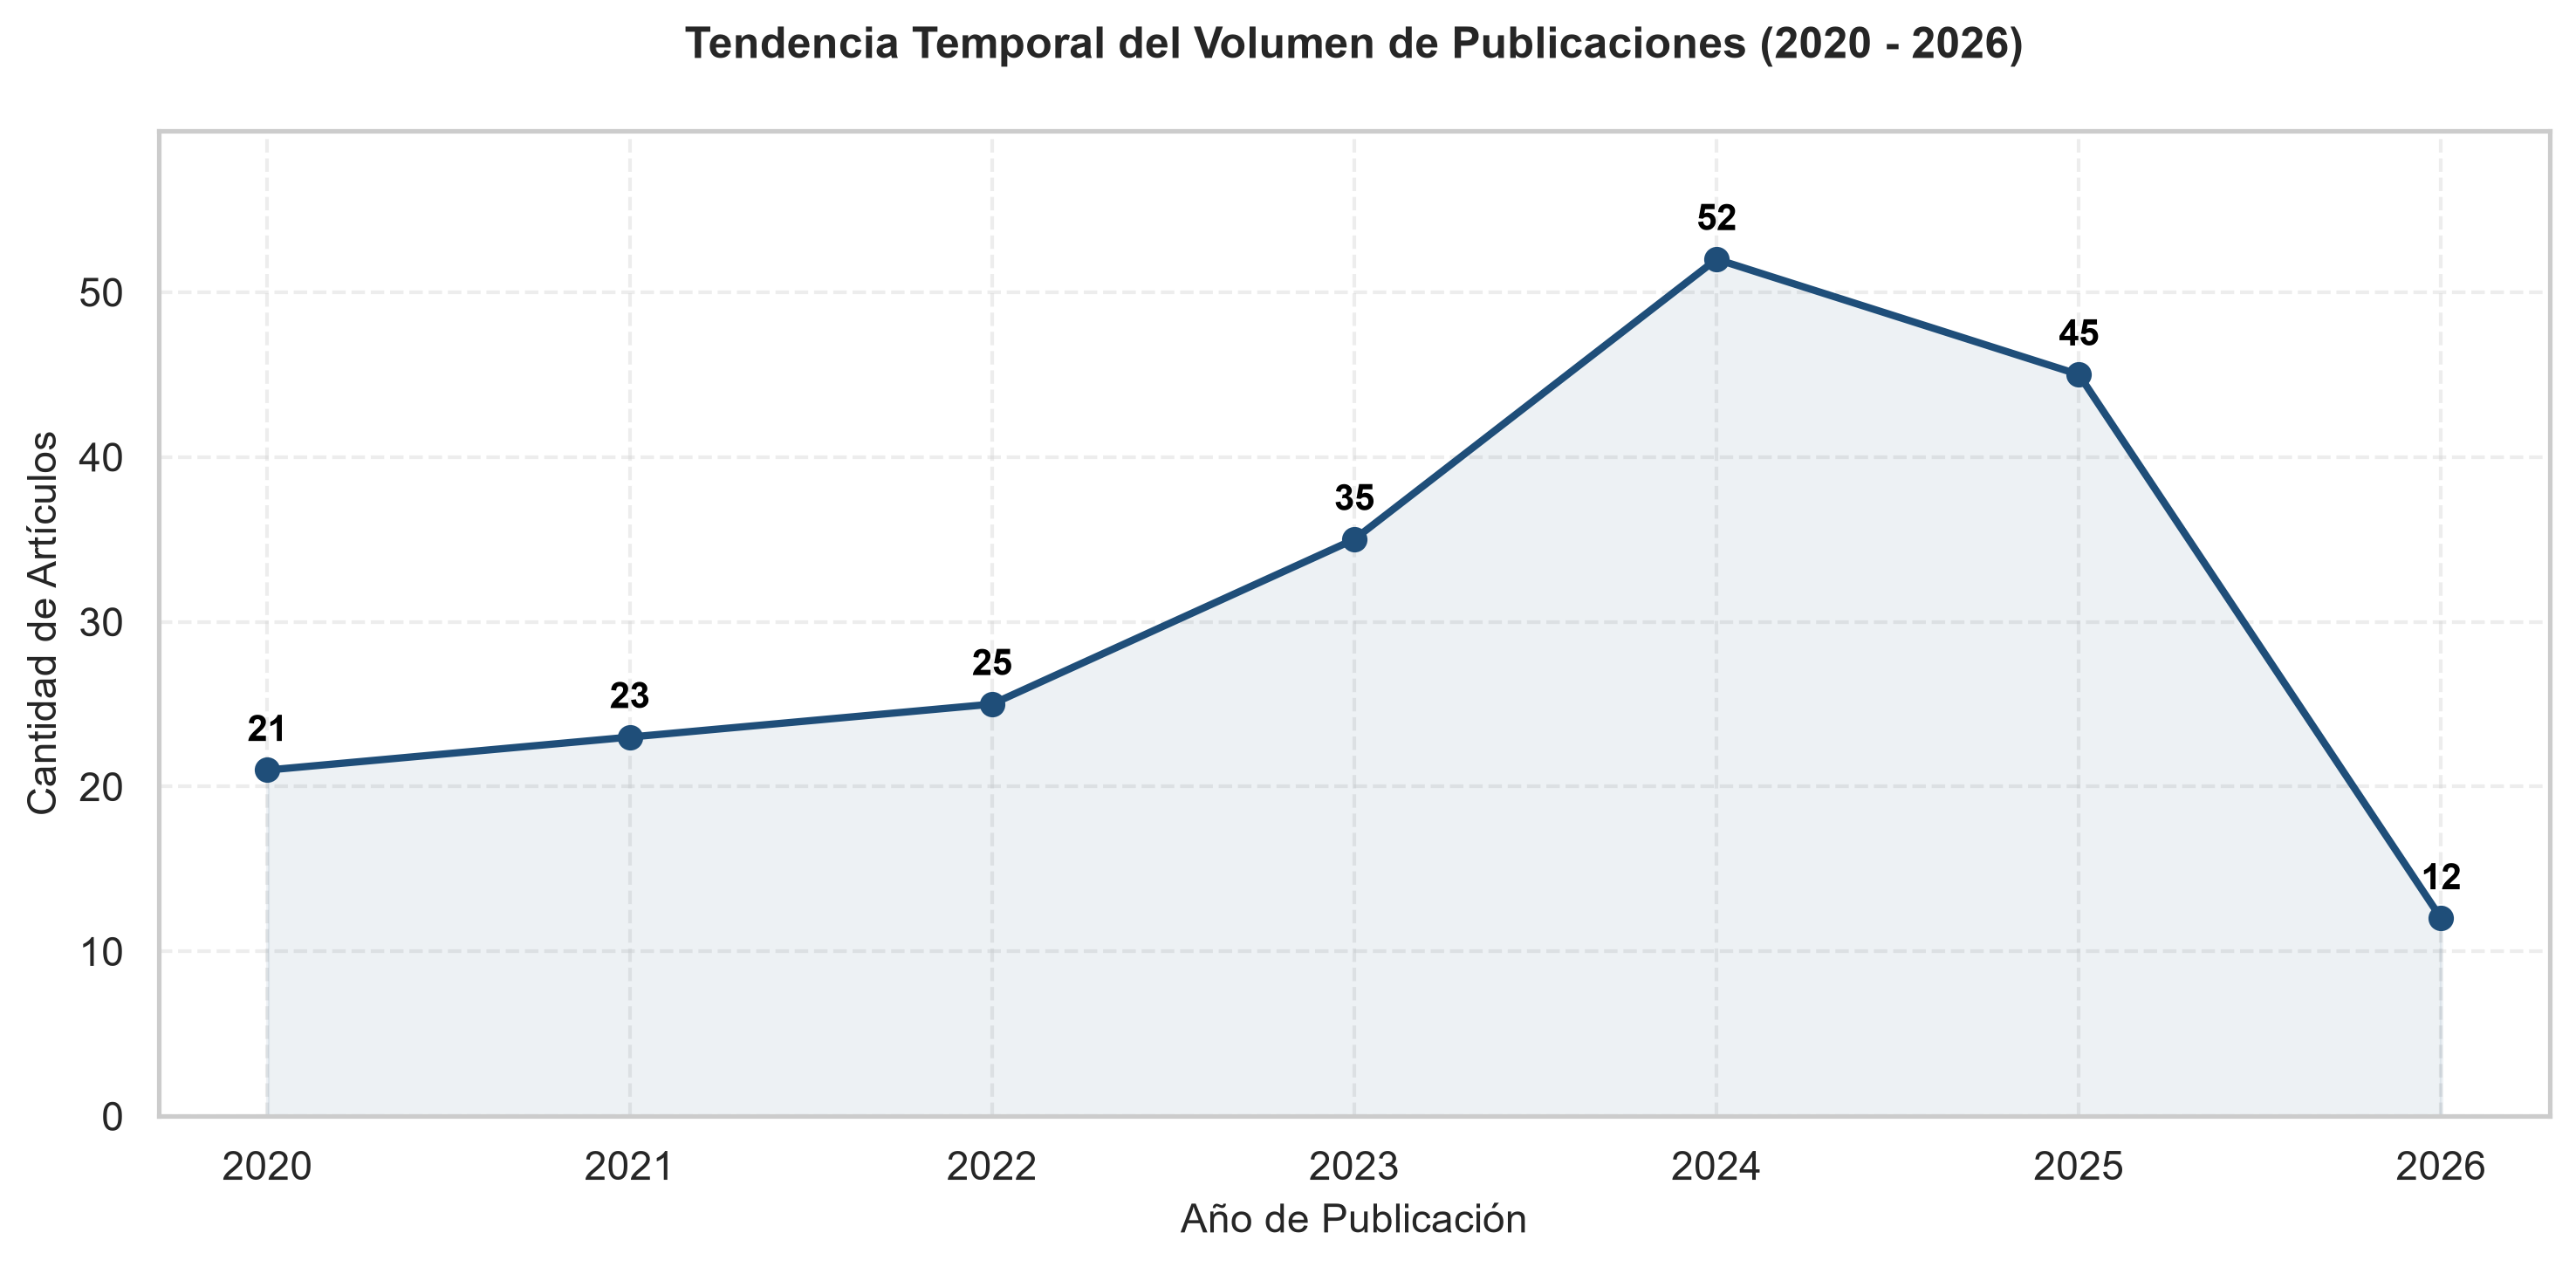
\includegraphics[width=0.48\textwidth]{../graficos/23_linea_publicaciones_año.png}}
\caption{Línea de Tendencia: Volumen Temporal de Publicaciones Científicas (2020--2026).}
\label{fig:linea_publicaciones}
\end{figure}

\begin{table}[htbp]
\centering
\renewcommand{\arraystretch}{1.2}
\caption{Distribución de Publicaciones Analizadas por Año}
\label{tab:dist_anos}
\begin{tabular}{cc}
\toprule
\textbf{Año de Publicación} & \textbf{Cantidad de Artículos} \\
\midrule
2020 & 21 \\
2021 & 23 \\
2022 & 25 \\
2023 & 35 \\
2024 & 52 \\
2025 & 45 \\
2026 & 12 \\
\bottomrule
\end{tabular}
\end{table}


Este crecimiento exponencial se alinea con la maduración de los frameworks de programación de deep learning como PyTorch y TensorFlow, que han facilitado enormemente la experimentación y despliegue rápido de modelos de visión compleja por parte de grupos de investigación en todo el mundo.

\subsection{Canales de Difusión y Venues Principales}
El análisis de los canales de publicación revela un corpus altamente consolidado en publicaciones de calidad. De los 213 artículos analizados, 175 corresponden a artículos de revistas científicas de alto impacto (journals) y 38 a contribuciones presentadas en conferencias internacionales de prestigio, destacando la marcada presencia de revistas líderes en el área como \textit{IEEE Transactions on Intelligent Transportation Systems} y \textit{Sensors}. La concentración en estas revistas y congresos especializados subraya la solidez científica del corpus analizado y asegura la relevancia técnica de las tendencias estadísticas y metodológicas que se derivan de la presente revisión.

\subsection{Clasificación de Enfoques de Inteligencia Artificial}
Para analizar la evolución de las técnicas de IA, los artículos han sido clasificados en cuatro categorías principales basadas en la descripción de sus algoritmos:
\begin{itemize}
    \item \textbf{Deep Learning (DL):} Trabajos fundamentados en redes neuronales convolucionales (CNN), modelos YOLO, redes de memoria a largo y corto plazo (LSTM) y arquitecturas de Transformers de visión (ViT), representando la gran mayoría de las propuestas debido a su capacidad para procesar datos no estructurados de alta dimensión.
    \item \textbf{Machine Learning (ML):} Algoritmos tradicionales de aprendizaje automático como máquinas de soporte vectorial (SVM), bosques aleatorios (Random Forest), K-vecinos cercanos (KNN) o modelos bayesianos.
    \item \textbf{Híbrido (ML + DL):} Estudios que integran representaciones de características de Deep Learning con clasificadores tradicionales de Machine Learning para optimizar el rendimiento y reducir el tiempo de entrenamiento.
    \item \textbf{Visión por Computadora Tradicional:} Propuestas basadas puramente en procesamiento de imágenes digital básico o descriptores geométricos mediante librerías como OpenCV tradicional sin el entrenamiento de modelos predictivos complejos.
\end{itemize}

La Tabla~\ref{tab:dist_metodologias} detalla la distribución cuantitativa de estos enfoques dentro del corpus.

\begin{table}[htbp]
\centering
\renewcommand{\arraystretch}{1.2}
\caption{Distribución por Enfoque Metodológico}
\label{tab:dist_metodologias}
\begin{tabular}{lc}
\toprule
\textbf{Enfoque Metodológico} & \textbf{Cantidad de Artículos} \\
\midrule
Deep Learning (DL) & 135 \\
Otros / No especificado & 44 \\
Híbrido (ML + DL) & 23 \\
Machine Learning (ML) & 11 \\
\bottomrule
\end{tabular}
\end{table}


La Fig.~\ref{fig:cruce_metodologias_entornos} ilustra la correlación existente entre los enfoques metodológicos adoptados y los entornos experimentales en los que se validan las soluciones. Como se aprecia, existe una clara preferencia por validar los modelos de Deep Learning en entornos de CCTV y escenarios reales de vía pública.

\begin{figure}[htbp]
\centerline{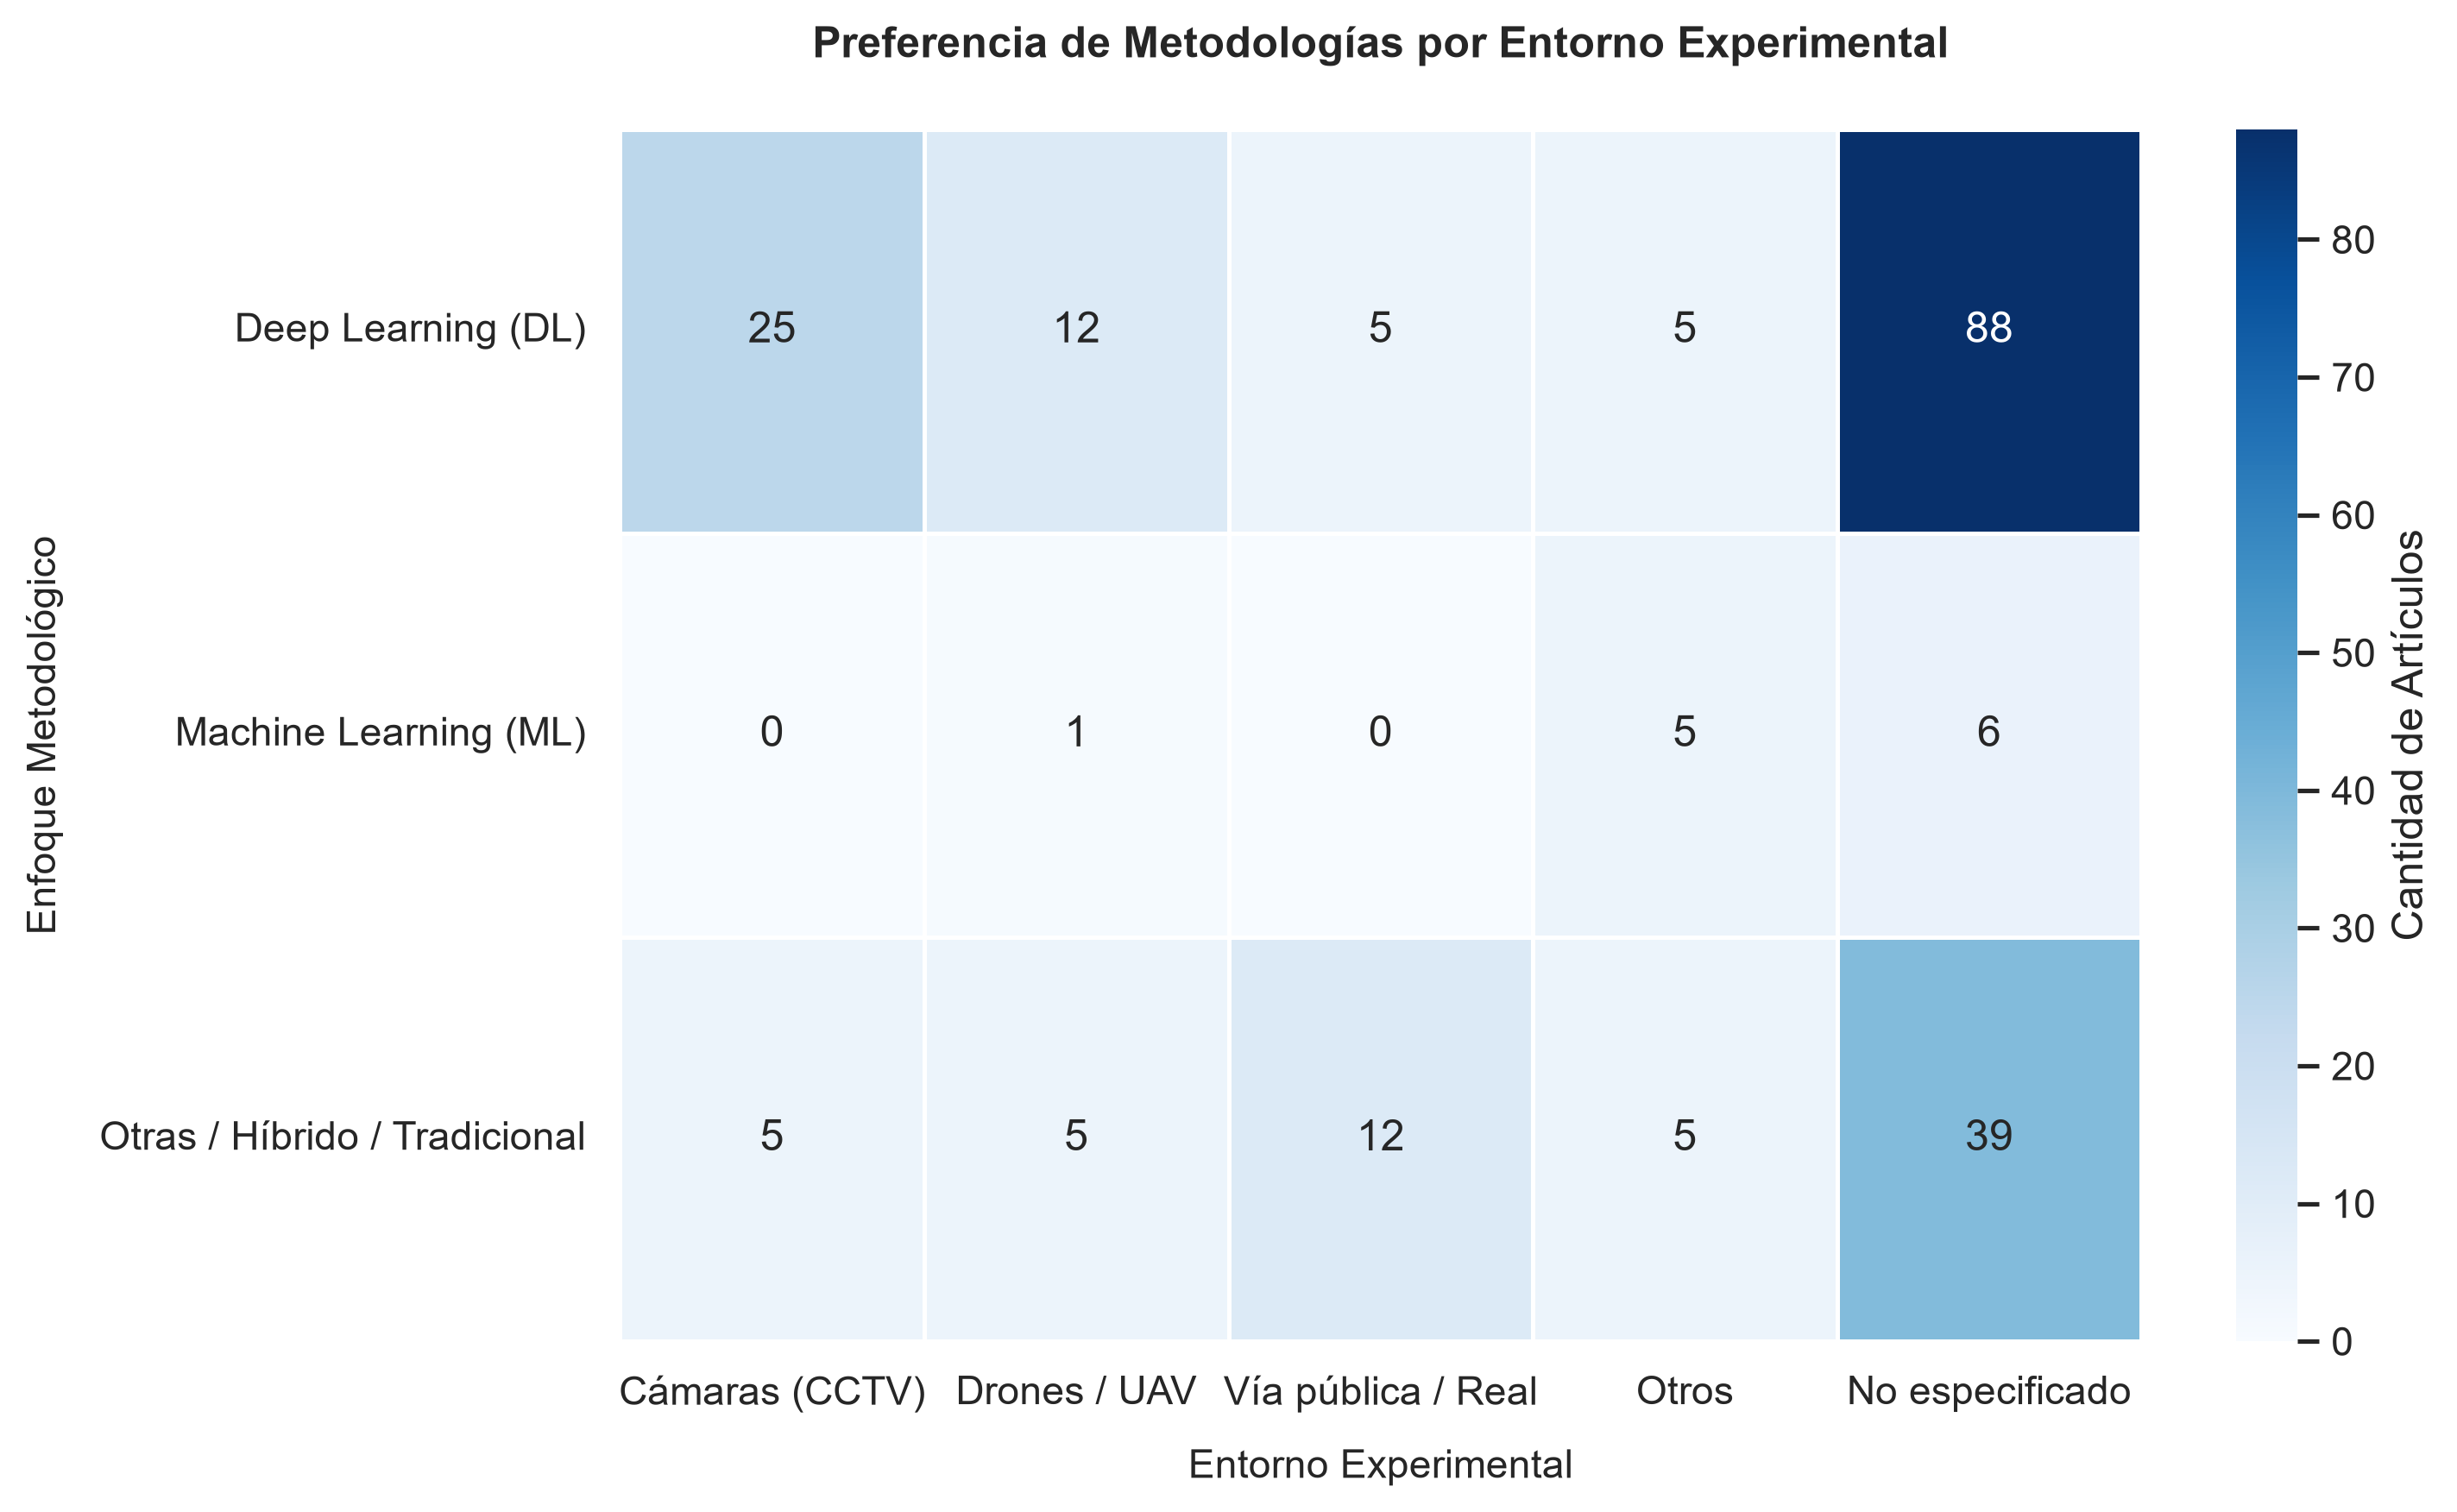
\includegraphics[width=0.48\textwidth]{../graficos/16_heatmap_cruce_3x3_entornos.png}}
\caption{Preferencia de Metodologías por Entorno Experimental (Distribución porcentual).}
\label{fig:cruce_metodologias_entornos}
\end{figure}
